In this chapter, we overview specifics of Ring-$\mathrm{LWE}$ based protocols which includes: methods of error sampling, methods to generate shared polynomial between two parties and performance analysis. The goal of this chapter is to explain in details how key-exchange reconciliations that was discussed in previous chapter was implemented as a protocol.


\section{Error sampling algorithm}
Lattice based cryptography began with the seminal work of Ajtai, who built a one-way function based on the worst-case hardness based on certain lattice problems \cite{ajtai1996generating}. These lattice problems are believed to be hard even in the presence of large quantum computers and such a promising post-quantum replacement for standard cryptography. The most general public key primitives like encryption schemes \cite{cryptoeprint:2012:230} and digital signatures \cite{cryptoeprint:2011:537} already have practical lattice based instantiations.

Many recent lattice based schemes require sampling from discrete Gaussian. The parameters of discrete Gaussian are governed by the security proofs of the particular schemes. A finite machine cannot sample from a discrete Gaussian distribution, hence one has to sample from a distribution close to it. It is a common practice to require that the statistical distance of the sampled distribution from the desired discrete Gaussian be less than $2^{-100}$.

Computing the probabilities requires floating point operations of at least $100$ bit precision if one wants to achieve a statistical distance less than $2^{-100}$ \cite{Janos2014}. Whereas any precomputation means storing a variable amount of values of the same precision. This can highly affect the sampling performance on personal computers and even make the implementation completely impractical on constrained devices. Weiden et al. \cite{cryptoeprint:2013:065} report that the Gaussian sampling takes up 50\% of the running time of Lyubashevsky's signature scheme (also known as BLISS) \cite{cryptoeprint:2011:537}. Thus efficient sampling from discrete Gaussians plays a crucial role in the performance
of these primitives.

S. Galbraith in \cite{Dwarakanath:2014:SDG:2635676.2635683} discussed different discrete Gaussian sampling algorithms suitable for constrained devices. By a constrained device we can think of an embedded or portable device with a small amount of memory (measured in kilobytes instead of gigabytes) and a modest processor that has to be economical with respect to power usage. Also these kind of devices do not necessarily come with floating point arithmetic capability. Even if a platform provides floating point arithmetic, the required precision is usually not supported natively. This means that software libraries have to be used for this functionality, and these can significantly worsen performance and take up additional space in the already tight memory.

A particular discrete Gaussian samplers may apply different techniques to increase the performance and reduce or even avoid the floating point operations, which usually utilize precomputed tables, hence not requiring floating point arithmetic. Many factors can affect the performance and memory consumption (i.e., the size and number of the potential precomputed tables). Such factors are the size of the Gaussian parameter, whether the center is zero or not, and whether the parameters are fixed or changing (or more precisely, the number of the needed parameter combinations). To evaluate the practicality of the discrete Gaussian samplers in lattice based cryptography one needs to assess the parameters of the distributions required by the different cryptographic
schemes.

The techniques utilized by different samplers require various amount of memory and floating point operations, which results in different overall performance on the particular platforms. Thus for the evaluation of their practical performance one needs to collect the characteristics of the discrete Gaussian samplers too.

% \begin{definition}
% \normalfont
% Discrete probability function (or PDF), $p(x)$, is a function that satisfies the following properties.

% \begin{enumerate}
%     \item Let $X$ be a discrete random variables. The probability that $x$ can take a specific value is $p(x)$. That is: $P[X=x]=p(x)$
%     \item $p(x)$ is non-negative for all real $x$
%     \item The sum of $p(x)$ over all possible values of $x$ is $1$, that is $\sum_{j} p_{j} = 1$ where $j$ represents all possible values that $x$ can have and $p_j$ is the probability at $x_j$
% \end{enumerate}
% \end{definition}

% One consequence of properties ($2$) and ($3$) is that $0 \le p(x) \le 1$. What it actually means is that discrete probability function is a function that can take a discrete number of values (not necessarily finite). This is most often the non-negative integers or some subset of the non-negative integers. There is no mathematical restriction that discrete probability functions only be defined at integers, but in practice this is usually what makes sense. Each of the discrete values has a certain probability of occurrence that is between zero and one. That is, a discrete function that allows negative values or values greater than one is not a probability function. The condition that the probabilities sum to one means that at least one of the values has to occur.

% \begin{definition}
% \normalfont
% The cumulative distribution function ($\mathrm{CDF}$) is the probability that the variable takes a value less than or equal to $x$. That is: $Pr[X \le x]= \alpha$. For a discrete distribution, the $\mathrm{CDF}$ can be expressed as: $\sum_{i = 0}^{x}f(i)$
% \end{definition}

In the following by PDF and CDF we are referring to \textit{Probability Density Function} and \textit{Cumulative Distribution Function}. Note that the relation between the probability density function $f$ and the cumulative distribution function $F$ is $F(k) = \sum_{i \le k} f(i)$ if $f$ is discrete and  $F(x) = \int_{y \le x} f(y)\,dy$ if $f$ is continuous.



\begin{definition}
\normalfont
The probability density of the normal distribution is:
$f(x\;|\;\mu ,\sigma ^{2})={\frac {1}{\sqrt {2\sigma ^{2}\pi }}}\;e^{-{\frac {(x-\mu )^{2}}{2\sigma ^{2}}}}$

Where:
\begin{itemize}
    \item $\mu$ is mean or expectation of the distribution (center of $\mathrm{PDF}$)
    \item $\sigma$ is standard deviation
    \item $\sigma^{2}$ is variance
\end{itemize}
\end{definition}

\begin{plain}
\normalfont
Coefficients of polynomials in Ring-$\mathrm{LWE}$ are $\in \mathbb{Z}$. Therefore, error sampling methods should sample from \textit{Discrete Distributions} as oppose to \textit{Continuous Distributions}.
\end{plain}

\subsection{Inversion sampling}
Inverse transform sampling (also known as Smirnov transform) is a basic method for pseudo-random number sampling, i.e. for generating sample numbers at random from any probability distribution given its cumulative distribution function.

Inverse transformation sampling takes uniform samples of a number $u$ between $0$ and $1$, interpreted as a probability, and then returns the largest number $x$ from the domain of the distribution $P(X)$ such that $P(-\infty <X<x)\leq u$.

In this method, we are randomly choosing a proportion of the area under the curve and returning the number in the domain such that exactly this proportion of the area occurs to the left of that number. Intuitively, we are unlikely to choose a number in the far end of tails because there is very little area in them which would require choosing a number very close to zero or one.

Computationally, this method involves computing the quantile function of the distribution; in other words, computing the cumulative distribution function ($\mathrm{CDF}$) of the distribution (which maps a number in the domain to a probability between $0$ and $1$) and then inverting that function. This is the source of the term \quotes{inverse} or \quotes{inversion} in most of the names for this method. Note that for a discrete distribution, computing the CDF is not in general too difficult: we simply add up the individual probabilities for the various points of the distribution. For a continuous distribution, however, we need to integrate the probability density function ($\mathrm{PDF}$) of the distribution, which is impossible to do analytically for most distributions including the normal distribution. As a result, this method may be computationally inefficient for many distributions and other methods are preferred.

For the normal distribution, the lack of an analytical expression for the corresponding quantile function means that other methods may be preferred computationally. It is often the case that, even for simple distributions, the inverse transform sampling method can be improved on, for example, the ziggurat algorithm and rejection sampling \cite{Janos2014}.

\subsubsection{Naive sampling approach using \texorpdfstring{$\mathrm{PDF}$}{PDF} function}
One simple approach which generates only positive integer samples is calculating probabilities using $\mathrm{PDF}(x)$ $\forall x \in [0, \text{variance}]$ and putting them in an array. Note that, sum of probability array would not be equal to one because we ignored the probabilities of negative values. Thereafter, we need to normalize the probability array such that sum would equal to $1$. Then, create a new array with the same size as probability array but setting first element of new array as first element of probability array. Thereafter, we set new array at any index to sum of probability array until that index. We can call the probability array, vector of $\mathrm{PDF}$ values and also call second array, vector of $\mathrm{CDF}$ values. Note that value of last element of $\mathrm{CDF}$ vector should equal to $1$ because we normalized the probability list and sum of probability list should equal to $1$. 

To sample integers in range $[0, \text{variance}]$ using this method, simply generate a random number between $[0, 1)$ uniformly at random, lets call it $u$. Then find a index such that $u < \mathrm{CDF}[index]$. The value of \textit{index} is a sample from the distribution.

Below is an implementation of the naive Gaussian sampler that we described above; centered at $0$ with $\sigma = \frac{8}{\sqrt{2  \pi}}$ as suggested in early draft of $\mathrm{BCNS}$ protocol.



\begin{algorithm}[H]
    \caption{naive Gaussian sampler by estimating cdf values}
    \begin{algorithmic}[1]
        \State sigma $\gets 8 / \sqrt{2  \pi}$ 
        \State variance $\gets \text{sigma}^2$
        \State mu $\gets 0$
        \State domain $\gets$ $\lceil\text{variance}\rceil$
        \item[] \Comment{probability density of the normal distribution}
        \Function{pdf}{x}
            \State \textbf{return:} $(1/\sqrt{2 \pi \times \text{variance}}) \times e^{-{(x - \text{mu})}^2 / (2 \times \text{variance})}$
        \EndFunction
        \item[] \Comment{note that sum of probabilities that this function generates is equal to 1/2}
        \item[] \Comment{because we are ignoring probabilities of negative numbers}
        \Function{create\_pdf\_vector}{}
            \State pdf\_vector $\gets$ empty array of size $=$ domain
            \For{ $x \gets 0 \text{ to domain}$ }
                \State pdf\_vector[x] $\gets$ pdf(x)
            \EndFor
            \State \textbf{return:} pdf\_vector
        \EndFunction
        \item[] \Comment{normalize probability list such that sum of probability would equal to 1}
        \Function{normalize\_pdf\_vector}{pdf\_vector}
            \State $s \gets$ sum(pdf\_vector)
            \For{ $i \gets 0 \text{ to domain}$ }
                \State pdf\_vector[$i$] = pdf\_vector[$i$] $/ \text{sum}$ 
                \State $i \gets i + 1$
            \EndFor
            \State \textbf{return:} pdf\_vector
        \EndFunction
        \item[] \Comment{create cdf vector from pdf\_vector}
        \Function{create\_cdf\_vector}{pdf\_vector}
            \State cdf\_vector $\gets$ empty array of size $=$ domain
            \State total $\gets 0$
            \For{ $i \gets 0 \text{ to } \text{domain}$ }
                \State total $\gets$ total + pdf\_vector[$i$]
                \State cdf\_vector[$i$] $\gets$ total
            \EndFor
            \State \textbf{return:} cdf\_vector
        \EndFunction
        \algstore{example1}
    \end{algorithmic}
\end{algorithm}

\begin{algorithm}[H]
    \begin{algorithmic}
        \algrestore{example1}
        \item[] \Comment{sample from cdf\_vector}
        \Function{sample}{}
            \State rand $\gets$ select a number in range $[0, 1)$ uniformly random
            \State index $\gets 0$
            \While{ $\text{rand} > \text{cdf\_vector[index]}$ }
                \State index $\gets$ index $+ 1$
            \EndWhile
            \State \textbf{return:} index
        \EndFunction
        \item[] \Comment{initialize the sampler}
        \State pdf\_vector $\gets$ create\_pdf\_vector()
        \State pdf\_vector $\gets$ normalize\_pdf\_vector(pdf\_vector)
        \State cdf\_vector $\gets$ create\_cdf\_vector(pdf\_vector)
        \State s $\gets$ sample(cdf\_vector)
    \end{algorithmic}
\end{algorithm}

\iftoggle{verylong}{
\lstinputlisting[language=Python, caption=Naive Gaussian sampler]{code_snippets/naive_gaussian_sampler.sage}
}{}

\begin{figure}[H]
\centering
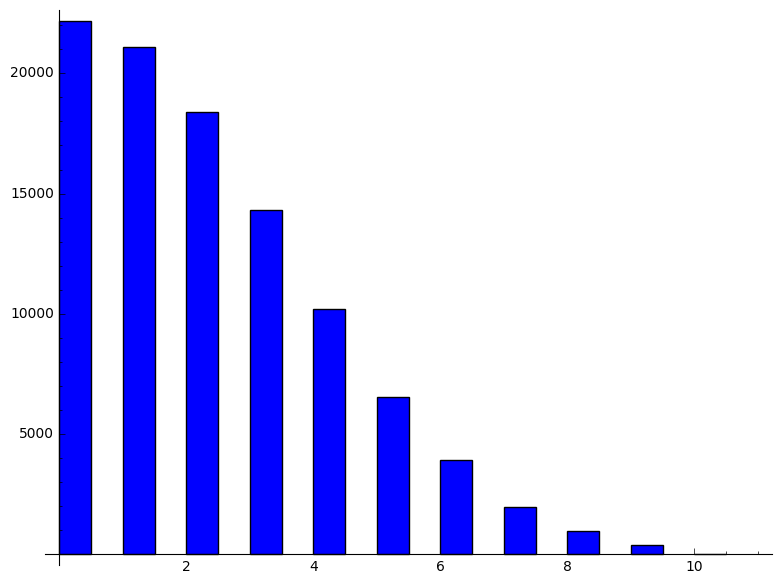
\includegraphics[scale=0.3]{naive-samples}
\caption{Plot (or histogram) of Gaussian samples using the naive method}
\figuresubtitle{Above is centered at $0$ and $\sigma = \frac{8}{\sqrt{2  \pi}}$}
\end{figure}



\subsubsection{Inversion sampling using \texorpdfstring{$\mathrm{PDF}$}{PDF} function and bisection search}
Above method can be improved using Taylor approximation to estimate the $\mathrm{CDF}$ and bisection search to estimate the inverse of $\mathrm{CDF}$. It is important to note that $\mathrm{CDF}$ function of normal distribution is not invertible so to calculate the inverse of $\mathrm{CDF}$ function we need to use Taylor series to find the integral (or area under the graph) of $\mathrm{PDF}$ function.

The bisection search method is a root-finding method that repeatedly bisects an interval and then selects a sub-interval in which a root must lie for further processing. It is a very simple and robust method, but it is also relatively slow. Because of this, it is often used to obtain a rough approximation to a solution which is then used as a starting point for more rapidly converging methods. This method is also called the interval halving method. Bisection search method does not really takes the advantage of the fact that coefficients of error polynomial are integers, so we need to round the sample to nearest integer which is not the most efficient approach. Also, to calculate the inverse of $\mathrm{CDF}$ we are constantly calculating $\mathrm{CDF}$ and also so we are not storing the $\mathrm{CDF}$ values (memorizing concept) of particular probability. As a result, this approach is very slow.


\begin{algorithm}[H]
    \caption{Gaussian sampler using Taylor series and bisection search}
    \begin{algorithmic}[1]
        \State sigma $\leftarrow 8 / \sqrt{2  \pi}$, variance $\leftarrow \text{sigma}^2$
        \item[] \Comment{probability density of the normal distribution}
        \Function{pdf}{x}
            \Return $(1/\sqrt{2 \pi \times \text{variance}}) \times e^{-{(x - \text{mu})}^2 / (2 \times \text{variance})}$
        \EndFunction
        \item[] \Comment{calculates cumulative distribution using Taylor approximation}
        \Function{cdf}{x}
            \If{x $<$ -1 $\times$ variance}
                \Return 0.0
            \ElsIf{x $>$ variance}
                \Return 1.0
            \EndIf
            \State sum $\leftarrow$ 0.0
            \State term $\leftarrow x$
            \State $i \leftarrow 3$
            \While{sum + term $\neq$ sum}
                \State sum $\leftarrow$ sum + term
                \State term $\leftarrow$ term $\times x^2 / i$
                \State $i \leftarrow i + 2$
            \EndWhile
            \Return $0.5 + $ sum $\times$ pdf(x)
        \EndFunction
        \item[] \Comment{bisection search to find a value $y$ such that it's CDF equals to $x$}
        \Function{inverse\_cdf}{x, delta, lo, hi}
            \State mid $\leftarrow$ lo $+$ (hi $-$ lo) $/ 2$
            \If{hi $-$ lo $<$ delta} \Return mid
            \ElsIf{cdf(mid) $>$ x}
                \State \Return inverse\_cdf(x, delta, lo, mid)
            \Else \text{ }
                \State \Return inverse\_cdf(x, delta, mid, hi)
            \EndIf
        \EndFunction
        \item[] \Comment{initialize the bisection search}
        \Function{inverse\_cdf\_init}{x}
            \State mid $\leftarrow$ lo $+$ (hi $-$ lo) $/ 2$
            \State \Return inverse\_cdf(x, 0.00000001, -variance, variance)
        \EndFunction
        \algstore{example2}
    \end{algorithmic}
\end{algorithm}



\begin{algorithm}[H]
    \begin{algorithmic}
        \algrestore{example2}
        \item[] \Comment{sample from Gaussian by generating a random number and find it's inverse of CDF}
        \Function{sample}{}
            \State $x \leftarrow $ generate a number between $[0, 1)$ uniformly random
            \State \Return inverse\_cdf(x, variance)
        \EndFunction
        \item[] \Comment{initialize the sampler}
        \State pdf\_vector $\leftarrow$ create\_pdf\_vector()
        \State pdf\_vector $\leftarrow$ normalize\_pdf\_vector(pdf\_vector)
        \State cdf\_vector $\leftarrow$ create\_cdf\_vector(pdf\_vector)
        \State s $\leftarrow$ sample(cdf\_vector)
    \end{algorithmic}
\end{algorithm}

\iftoggle{verylong}{
\lstinputlisting[language=Python, caption=Improved Gaussian sampler]{code_snippets/inversion_sampling_gaussian.sage}
}{}

\begin{figure}[H]
\centering
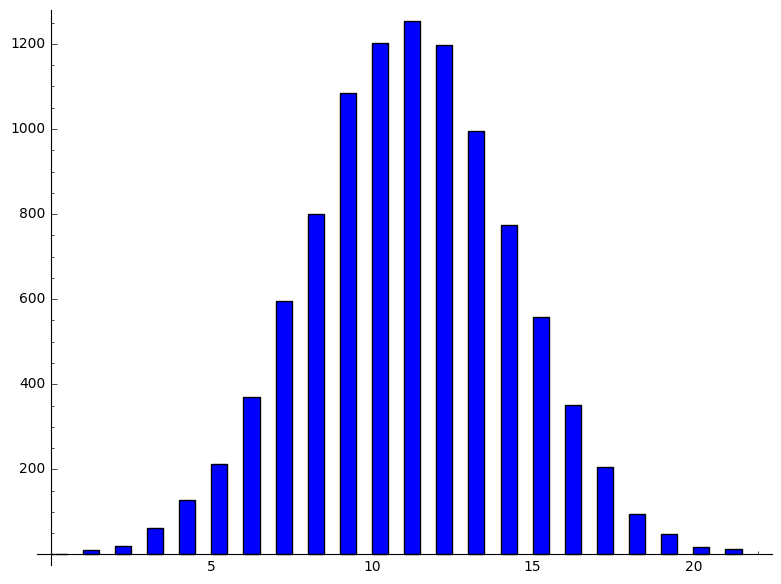
\includegraphics[scale=0.3]{improved_sampler}
\caption{Plot (or histogram) Gaussian sampler using bisection search and Taylor series}
\figuresubtitle{Above is centered at $\text{variance}^2$, $\sigma = \frac{8}{\sqrt{2  \pi}}$}
\end{figure}

\subsubsection{Inversion sampling using pre-calculated \texorpdfstring{$\mathrm{CDF}$}{CDF} table}
$\mathrm{BCNS}$ protocol uses inversion sampling with pre-computed look-up table of $\mathrm{CDF}$. If look-up table was not available, then we had to calculate the $\mathrm{CDF}$. The specification of $\mathrm{CDF}$ look-up table is the following:

\begin{equation}
    \begin{aligned}
        \text{table}[0] = 2^{189}  \\
        \text{table}[51] = 2^{192}\\
        \text{table}[i] < \text{table}[i+1] : \forall_{i} \in 0 \le i \le 50
    \end{aligned}
\end{equation}


To samples form this look-up table, we independently generate a $192$-bit integer $v_{j}$ uniformly at random, and compute the unique smallest integer index $ind_{j} \in [0, 50]$ such that $v_{j} < \text{table}[ind_{j}]$. We then generate one additional random bit to decide the sign $sign_{j} \in \{-1, 1\}$, and return the $j$-th coefficient as $s_{j} \leftarrow sign_{j} \times ind_{j}$. $\mathrm{BCNS}$ uses little Endian memory storing format (i.e. 192 bits stored as \texttt{struct} of $3 \times 64 = 192 $ bits) to store the array. Little endians in essence means storing the least significant byte in the smallest address.


\begin{algorithm}[H]
    \caption{gaussian sampler given CDF table as written in $\mathrm{BCNS}$ protocol}
    \begin{algorithmic}[1]
        \State rlwe\_table $\leftarrow$ $52 \times 3$ matrix of 64 bit little endians
        \State big\_integers $\leftarrow$ empty array with size equals to number of rows in rlwe\_table (i.e. 52)
        \item[] \Comment{convert little-endian as stored above to Big-endian}
        \Function{little\_to\_big\_endian}{}
            \For{$ i \gets 0 \text{ to } \text{height of rlwe\_table}$}
                \State big $\leftarrow 0$
                \For{$ j \gets 0 \text{ to } \text{width of rlwe\_table}$}
                    \State big $\leftarrow$ big \texttt{OR} (rlwe\_table[$i$][$j$] \texttt{LSHIFT} ($j \times 64$))
                \EndFor
                \State big\_integers[$i$] $\leftarrow$ big
            \EndFor
            \State \Return big\_integers
        \EndFunction
        \item[]
        \item[] \Comment{this function uses bits that are sampled uniformly at random to sample Gaussian}
        \Function{sample}{}
            \State $n \leftarrow $ get a 192 bits uniformly random
            \State $i \leftarrow 0$
            \For{$i \gets 0 \text{ to } \text{length(big\_integers)}$}
                \If{$n < $ big\_integers[$i$]}
                    \State \Return $i$
                \EndIf
            \EndFor
        \EndFunction
    \end{algorithmic}
\end{algorithm}

\iftoggle{verylong}{
\lstinputlisting[language=Python, caption=Gaussian sampler using pre-calculated table of CDF]{code_snippets/inversion_sampling_given_cdf.sage}
}{}

\begin{figure}[H]
\centering
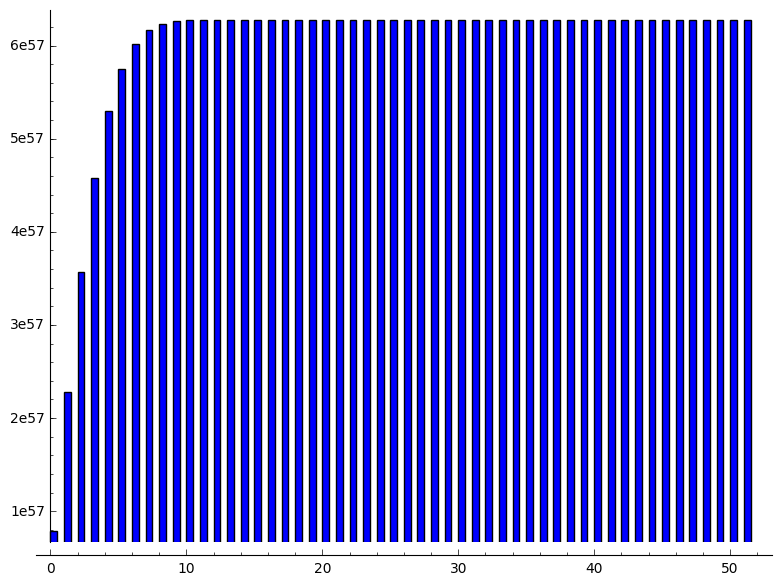
\includegraphics[scale=0.3]{cdf-table-BCNS.png}
\caption{Plot of precomputed $\mathrm{CDF}$ table as implemented in $\mathrm{BCNS}$ protocol}
\figuresubtitle{Notice the last column is just $1$s.}
\end{figure}


\begin{figure}[H]
\centering
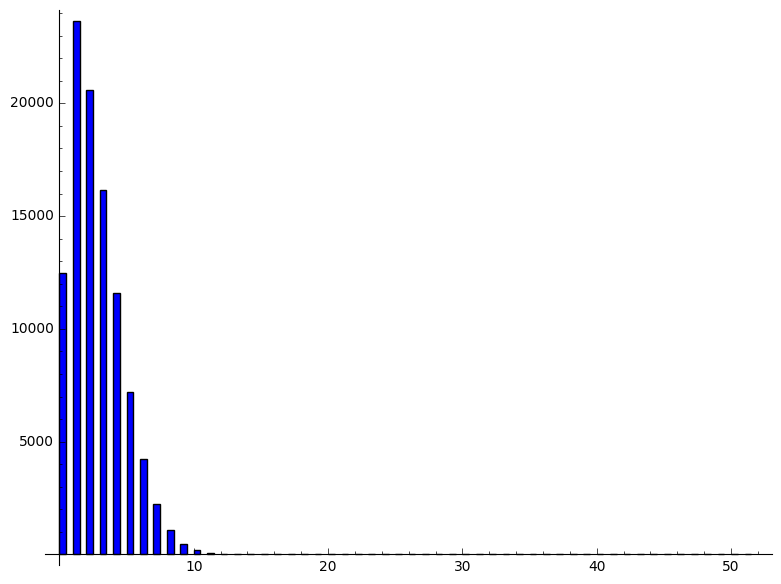
\includegraphics[scale=0.3]{samples-from-BCNS.png}
\caption{Plot (or histogram) of $\mathrm{BCNS}$ Gaussian sampler}
\figuresubtitle{Close to a perfect discrete Gaussian sampler (statistical difference $<2^{-128}$)}
\end{figure}




\subsection{Binomial distribution}
$\mathrm{NewHope}$ protocol uses binomial distribution ($\Psi_{16}$) as oppose to Gaussian distribution for efficiency reasons. Interestingly, difference of two independently uniformly sampled random variables is a binomial distribution sample when bits are uniformly sampled. The method they use is to sample $b$, $b'$ each $16$ bits, then their difference forms a binomial distribution sample centered at zero. This distribution has standard deviation $\sigma = \sqrt{\frac{k}{2}}$, where $k$ is number of bits. In the paper \cite{alkim2015post}, Alkim et al. provides a proof that such a binomial distribution is a good approximation of Gaussian distribution.  


\begin{figure}[H]
\centering
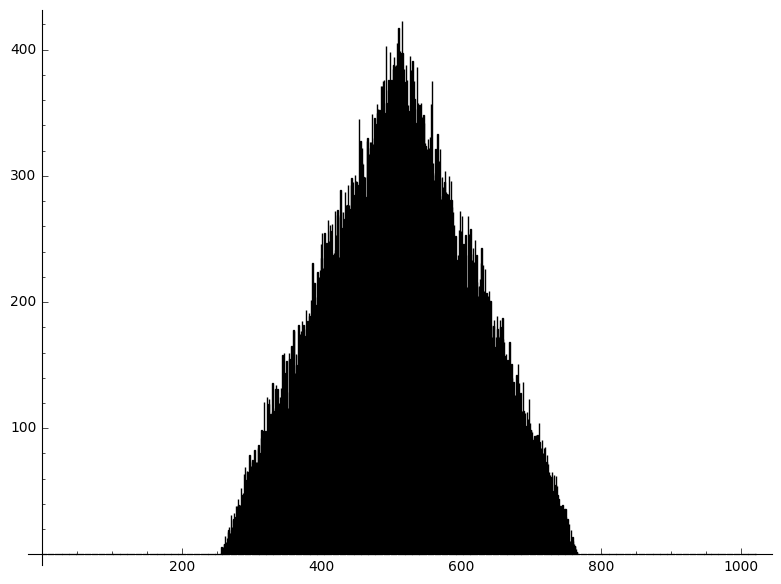
\includegraphics[scale=0.3]{binomial-distribution-shifted.png}
\caption{Plot of Binomial distribution $\Psi_{8}$, shifted for visualization purposes}
\figuresubtitle{This binomial distribution would have a standard deviation of $\sigma = \sqrt{\frac{8}{2}}$}
\end{figure}


\begin{algorithm}[H]
    \begin{algorithmic}[1]
        \caption{Binomial distribution sampler with $\Psi_{16}$ as written in $\mathrm{NewHope}$ protocol}
        \item[] \Comment{generate two 16 bit uniformly random number return their difference}
        \Function{sample}{big\_integers}
            \State $x \gets $ generate a 16 bits number uniformly random
            \State $y \gets $ generate a 16 bits number uniformly random
            \State \textbf{return:} $x - y$
        \EndFunction
    \end{algorithmic}
\end{algorithm}

\iftoggle{verylong}{
\lstinputlisting[language=Python, caption=Binomial distribution sampler with $\Psi_{8}$]{code_snippets/binomial_sampler.sage}
}{}
